\documentclass[11pt,a4paper,twoside]{article}
\usepackage{tascar}
\pagenumbering{arabic}
\pagestyle{empty}
\showtutorialtrue
\begin{document}
\setcounter{tutorial}{0}
\begin{tutorial}{Sensors, data logging and the lab streaming layer}{Gesture lab}
This tutorial is about collecting data from external sensors using
\tascar{} and lab streaming layer.
%
In this tutorial you will learn how to use head tracking,
electro-oculography (EOG) and video recordings in \tascar{}
environments.
%
Learn how \tascar{} communicates with lab streaming layer and about
the different types of data streams.
%
At the end you will be able to use \tascar{} data logging for the
recording of synchronised sensor data.

  \begin{learnitems}
  \item How to use head tracking, EOG and video recordings
  \item Communication between \tascar{} and lab streaming layer
  \end{learnitems}

  \begin{appitems}
  \item Recording of synchronised sensor data
  \end{appitems}

  \centerline{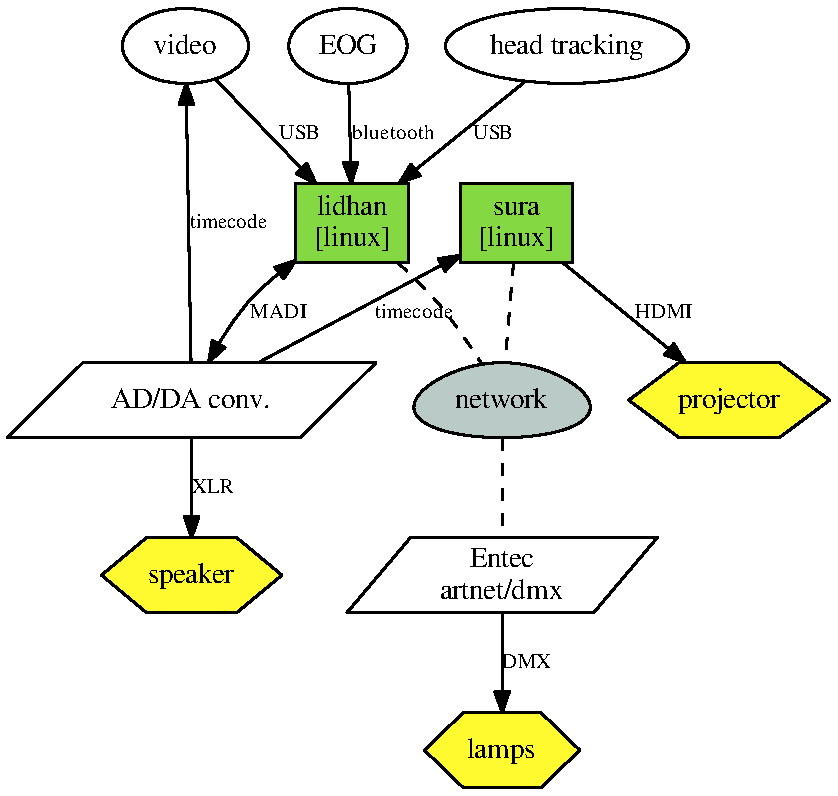
\includegraphics[width=0.5\columnwidth]{tutorial1_hardware}}
\end{tutorial}

\ifshowtutorial

\begin{itemize}
\item Make a copy of file {\tt cafeteria.tsc} in text editor.

\item Find {\tt <glabsensors.../>} module in the scene definition
  (see also manual). Have a look at the sensors in Gesture-lab -- what kind
  of information can they send?

\item To connect the bluetooth based EOG sensor make sure it is switched on. Then type in a terminal (before starting \tascar{}):

  {\tt sudo rfcomm connect 1}
  
  \begin{lstlisting}
    sudo rfcomm connect 1\end{lstlisting}
    
    If it displays {\tt Press CTRL-C for hangup} then everything should be fine -- otherwise ask Maartje, Giso, Jan, or Joanna.

  \item In the command line type \verb!tascar_lslsl!, which shows a list
    of LSL streams. What streams are available?
  \item Find \verb!<datalogging>...</datalogging>! external module
    (manual).  Set up the data logging for the EOG. Put in a Trial ID in the datalogging window and try recording for some time. Where is your data stored?
  \item The \verb!<datalogging>...</datalogging>! external module not only allows you to store data streams from sensors, 
but you can also send discrete variables as OSC messages. 
This could be useful when running an experiment script from Matlab. 
%
For example information about the subject behavior can be send as an
OSC message, so that later it can be seen exactly when an event
happened.
%
To do this, you have to define this variable in the datalogging
(manual), for example:
\verb! <variable path="/notfacingforward" size="1"/>!  To send the OSC
message from Matlab or from the terminal, for example type:
\begin{lstlisting} 
  send_osc( 'lidhan', 7777, '/notfacingforward', <number>); 
\end{lstlisting}
Try to define a boolean variable ``distracted'', which you will send while the experiment is running if the subject is distracted.
\item While the experiment is running, values of the data streams can
  also be accessed from Matlab and can be used to change experiment
  parameters.
  % 
  Have a look at the \verb!tutorial1.m! Matlab script that shows how
  to do this.
\item Be creative! Perform an experiment, during which the head and
  eye movements will be recorded. Try to change something based on the
  measured data in realtime.

  Include something about accessing data in realtime.
\end{itemize}
\fi
\end{document}
